\chapter{Introduction}
\label{sec:introduction}



The need and desire to faithfully reproduce the surrounding world using images is rooted deep in human nature. Images of our world have always played a fundamental role in human culture for telling stories, passing on knowledge and building visual maps of reality. Realistic images of the world are in essence a tool for humans to reflect upon it, learn from it and build ambitious new visions for it. There is a consistent line of development from cave and rock carvings dating back to 30,000 BC encompassing wall paintings and burial chambers in Egypt up to well reknown painters such as Da Vinci or Rembrandt. These works of art integrate elements of human expression that is the result of creative processes. However, there has also been the element of technique and understanding of nature, which was required to create realistic imagery. Painters such as Caspar David Friedrich would extensively study cloud shapes and cloud formations to be able to produce images of unprecedented realism.

With the computer, a completely new medium emerged, and with it a new methodology and way of thinking about realistic image creation. Crude rudimental rules, such as on aerial perspective by Leonardo Da Vinci~\cite{DaVinci1651}, evolved into highly accurate physical models and instead of a paint brush, numerical methods are employed to compute pixel colors which create an image. This is the domain of computer graphics, a branch in computer sciences, which aims to develop methods for the generation of photorealistic images from digital content and constantly tries to push the boundaries of what is technically possible.
\begin{figure}[ht]
\begin{center}
\resizebox{.98\textwidth}{!}{%
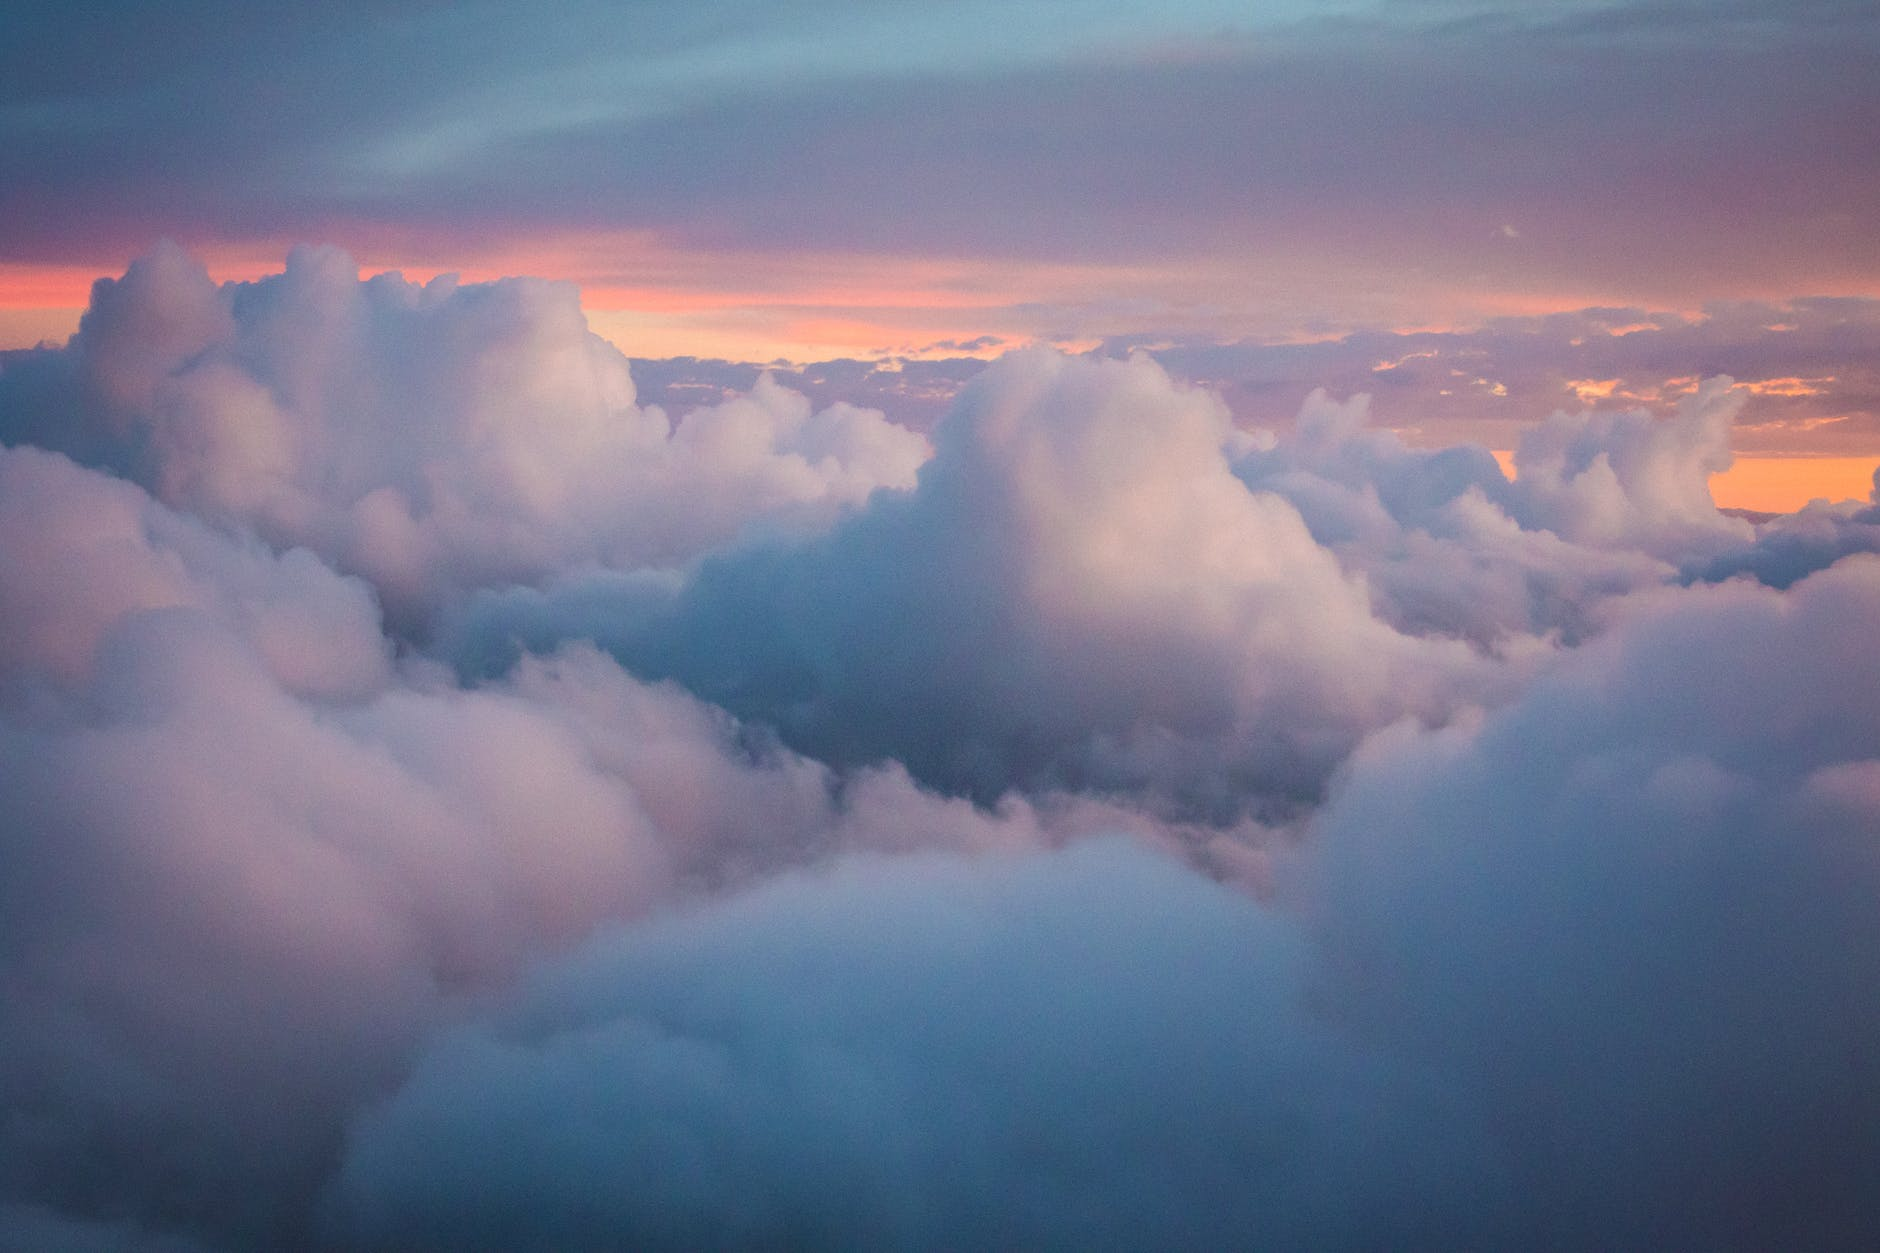
\includegraphics[height=3cm]{02_Introduction/images/clouds.jpg} %% Magda Ehlers
\hspace{0.01cm}
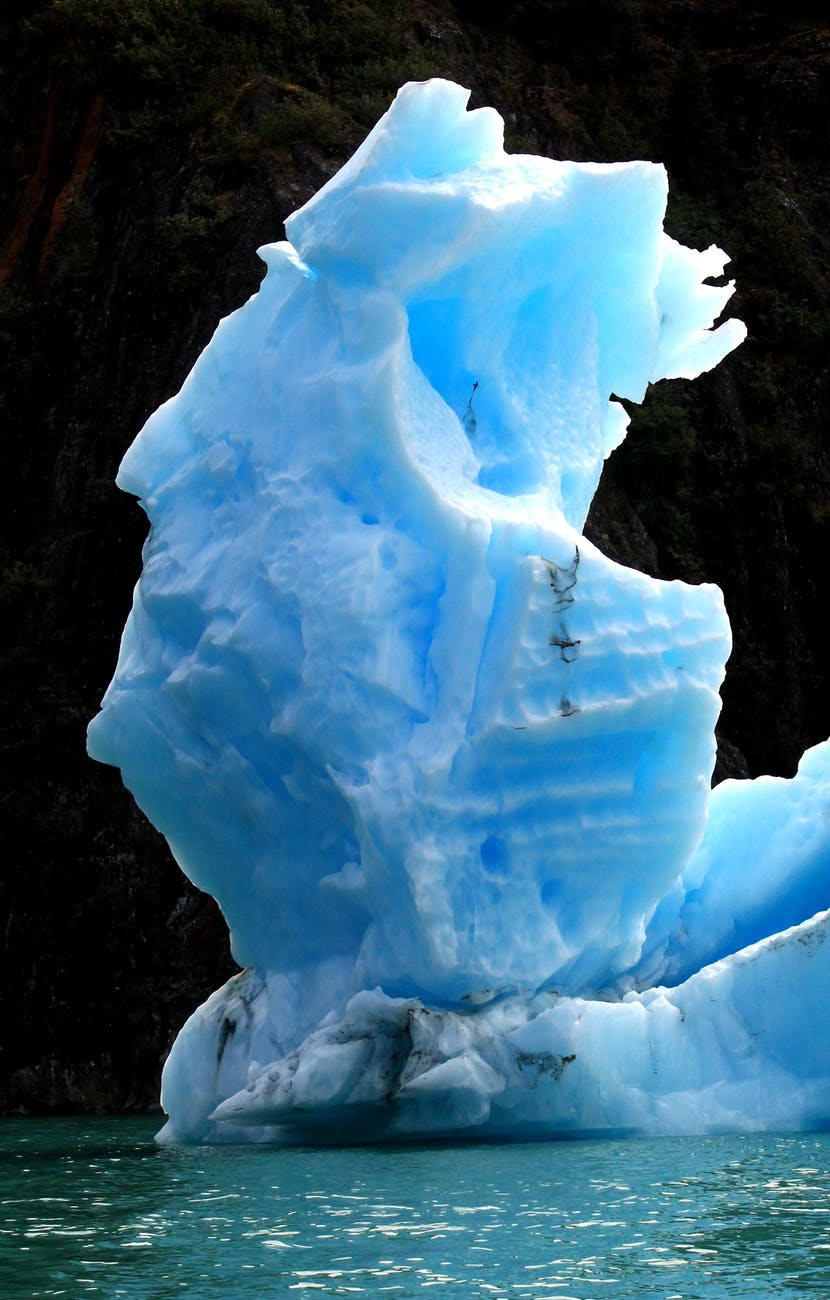
\includegraphics[height=3cm]{02_Introduction/images/iceberg.jpg} %% pixabay
\hspace{0.01cm}

\includegraphics[height=3cm]{02_Introduction/images/candle.jpg} %% Brett Sayles
}
\end{center}
\caption{Real world examples of participating media. Reproducing these optical phenomena with computers requires resource intensive light transport simulations for which deterministic methods are developed in this thesis\protect\footnotemark.}
\label{fig:intro_participating_media_examples}
\end{figure}

Computer generated imagery (CGI) is used widely across many domains and industries such as architecture, entertainment, advertising, automotive, manufacturing and scientific visualization, where each brings its own challenges with it. This high demand and wide adoption is why rendering in computer graphics is a heavily researched subject in industry and academia alike. The main challenge research in rendering is trying to address is the high amount of computation current algorithms require in order to generate realistic images. For example a single frame in an animation movie by Disney or Pixar takes multiple hours on average and much more in extreme cases. To produce all images for the whole movie, multiple computing centers with thousands of CPU cores are used, which requires substantial economical investments. One of the main efforts in rendering research therefore is to reduce the computational cost for realistic image generation.\footnotetext{Photos provided under Creative Commons CC0 license by  Magda Ehlers (clouds), pixabay (iceberg), Brett Sayles (candle).}

The advent of graphics computing hardware has paved the way for realtime applications. Here, together with some additional compromises in physical accuracy, incredible performance gains enable the generation of images in fractions of seconds and are the basis for new powerful interactive applications in the industries mentioned above. Finding methods that can generate results at interactive rates while allowing control, or at least understanding of accuracy losses, is another important research direction in graphics.

Computer hardware is ever-evolving\mydash while for a long time most of the increase in computing power came from higher density semiconductor fabrication\mydash this trend has almost come to a halt. Today, the growth in compute power is driven by parallelization on multi- and manycore systems. These challenges impact current rendering algorithms which mostly do not play well to the intricacies of the underlying hardware. While some first steps are being made in this direction (see for example Eisenacher et al.~\cite{Eisenacher13}), designing rendering algorithms that fully exploit the potential of next generation multi- or manycore hardware has been proclaimed as one of the future challenges for rendering by industry leaders (see Fascione~\cite{Fascione15}).

This thesis seeks to address these problems by following a trend which has been spurred by the so called physical based rendering revolution in graphics (see Keller et al.~\cite{Keller15}). In the early days of computer graphics, limitations in computing power required the use of cheap ad-hoc methods and other tricks to facilitate efficient image generation algorithms. With the growth in computational power, techniques and methods based on accurate physical models have become increasingly feasible and started replacing older heuristical approaches. Rendering became concerned with energy conservation, the use of correct physical quantities for describing the virtual scene and quantifiable error to physically correct ground truth results. Consistently adopting the framework provided by optical physics allowed rendering researchers to much better investigate and compare with work in other fields attacking very similar problems. While graphics research has always drawn inspiration and methods from other scientific domains, the emergence of physical based rendering caused a significant increase in research work which is based on findings and theories from other domains. Physics provided a common language allowing much easier to talk across disciplines.

In this spirit, this thesis investigates theories and methods from the astrophysics domain and nuclear sciences and adopts them for application in rendering. The resulting work presented in this thesis addresses all the three challenges mentioned above. Specifically, methods are presented which allow to reduce the computational cost for the demanding problem of rendering participating media such as clouds, smoke, fire, etc. and even allows\mydash with some compromise in accuracy\mydash applications at interactive rates. The methods devised in this thesis turn the rendering problem into the problem of solving a linear system of equations, exactly what high performance computing clusters (large scale many-core systems) have been designed for (see Koerner et al.~\cite{Koerner17}). This thesis constitutes a significant effort in putting forward an alternative approach to light transport simulation which has not seen a lot of attention lately but might have the potential to answer some of the research challenges in rendering today and tomorrow.

%\TD{visualization}
%\TD{inverse rendering}

\section{Research Questions}

This thesis is concerned with rendering volumetric media such as clouds, fire, milk, and fog which interacts with light. These participating media elements are ubiquitous in the real world and therefore also common in rendering. Today's standard methods in rendering operate by tracing particles of light (photons) through a given scene. These particles interact with the scene and form complex trajectories from light sources to the sensor of the virtual camera which captures the image. Participating media such as clouds or milk cause very long trajectories for light particles and therefore are computationally very demanding.


The problem of tracing particles through a participating medium which causes many particle interactions and long trajectories is not exclusive to simulation of light in computer graphics. Very similar problems exist in nuclear physics for example, when computing the dose of radiation leaving the protected core of a nuclear power plant. Here, high-energy neutrons are traced from the reaction through the surrounding wall, which acts as a participating medium (e.g. Haghighat et al.~\cite{Haghighat03}). In astrophysics, for example, the study of the formation of planets (which apparently to this day is not fully understood) has models that take the radiation of stars into account, and the associated simulation, therefore requires tracing particles that are emitted from fusion through clouds of debris and dust (see Armitage et al.~\cite{Armitage11}).

Common to all the problems mentioned above is the migration and interaction of particles or energy within a dense host medium. This is being described by linear transport theory, a field in mathematical physics, which is at the intersection between astrophysics, nuclear sciences and computer graphics.
\begin{figure}[ht]
\centering
%\missingfigure{linear transport as intersection between astrophysics nuclear sciences computer graphics }
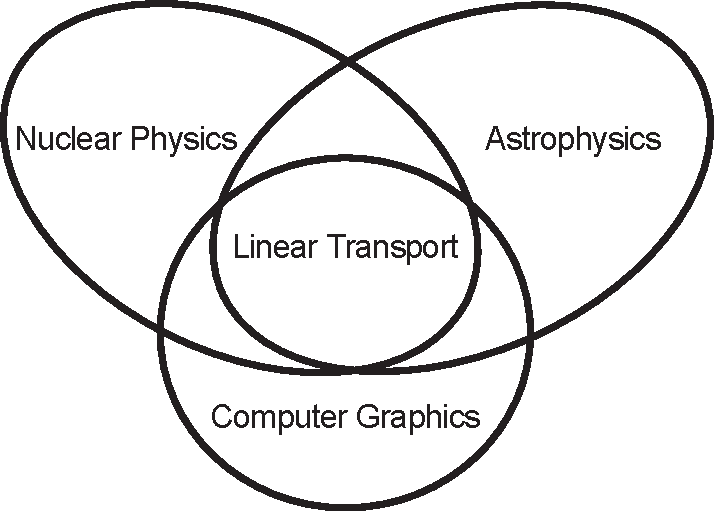
\includegraphics[width=0.6\textwidth]{02_Introduction/figures/fig_linear_transport.pdf}
\caption{Light transport simulation for rendering in graphics shares problems with other domains such as astrophysics and nuclear sciences. This thesis draws ideas from the long history of research done in those fields and inspires new methods for application in graphics.}
\label{fig:intro_linear_transport_fields}
\end{figure}

Now astrophysics and nuclear sciences have a much longer standing history than computer graphics and a lot of research was done before modern computers were widely available. This led to a large volume of work in those fields dealing with very similar problems in graphics from a very different perspective. As a result there are many interesting ideas, methods and techniques that can be adapted for applications in computer graphics.

D'Eon~\cite{DEon14} in his work explains vividly the challenges this type of research comes with. Starting with notation and terminology which makes it difficult to read and understand papers from these fields. Further many seminal texts from those other domains are out of print, expensive to aquire, lack offical digital distribution formats and generally are hard to find. Since much of academic research was published before modern computers became a commodity, most publications focus exclusively on theoretical treatments and simple one-dimensional or two-dimensional problems. Practical computational methods are lacking and simply were not focus of research back then. New methods will have to be devised after going through the literature and putting the puzzle pieces together. However, doing this type of translational research can lead to powerful new tools in graphics. Significant recent advances, such as the work by D'Eon et al.~\cite{dEon11}, Vorba et al.~\cite{Vorba16}, or Krivanek et al.~\cite{Krivanek14} are based to a large degree on old methods which were invented in other scientific domains.

Like the work mentioned above, this thesis follows the same spirit of adapting an existing method from another field for the application to image generation in computer graphics. The $P_N$-method (see Brunner~\cite{Brunner02}) is a very popular method in nuclear sciences. It allows to compute a global solution without using the computational demanding standard method of following particle trajectories. The classical diffusion approximation (see~Ishimaru~\cite{Ishimaru78}) is a method which is used in the astrophysics domain and actually has been introduced to graphics by Stam~\cite{Stam95}. However an extension to flux-limited diffusion was introduced in the astrophysics domain by Levermore et al.~\cite{Levermore81} and has not been introduced to graphics yet. What all these different methods have in common is the fact that they are based on a model that uses the same discretization in the angular domain.

The central research question this thesis will explore is whether these methods have merit for applications in computer graphics, and how they could be adopted to typical problems in rendering. This consists of two parts. First, the theory needs to be revisited and presented to a computer graphics audience. How is the theory derived from first order principles? Is it applicable for applications in rendering? What are the theoretical limitations and how do they affect the scope of applications? Second, modern and efficient methods need to be derived which allow application in a typical computer graphics context. How can the theoretical problem be solved for a typical application in rendering? How could a practical and efficient method look like? What shortcomings does it have and how could those be overcome?

\section{Summary of Original Contributions}

The research which was carried out as part of this thesis resulted in two major contributions, where one is based on the $P_N$-method popular in nuclear sciences and the other uses flux-limited diffusion from the field of astrophysics. In both cases practical methods for full three-dimensional problems did not exist and had to be devised, resulting in original published contributions in its own right.

\textbf{$P_N$-Method for Multiple Scattering in Participating Media~\cite{Koerner18}} The first contribution is a novel deterministic method for solving the $P_N$-equations on a finite difference grid for applications in rendering. The $P_N$-theory is derived and presented for a computer graphics audience. An original side product is a very concise and compact form of the real-valued $P_N$-equation which is new to the whole literature on $P_N$-based methods. The devised method introduced in this thesis is based on the idea of automated discretization. This approach works not only for the $P_N$-equations, but also for arbitrary potentially coupled PDE's and therefore has the potential to be of interest for other applications and problems in graphics. The $P_N$-method produces large systems of partial differencial equations which are well suited for being solved on a high performance computing cluster. An initial investigation into this direction was presented in \textbf{High-Performance Computing for Artistic Content Creation}~\cite{Koerner17}.

\textbf{Flux-limited Diffusion for Multiple Scattering in Participating Media~\cite{Koerner14}} The second contribution is a new and efficient method for computing the contribution of multiple scattered light in participating media. The method is based on flux-limited diffusion theory which is being derived and presented for a computer graphics audience. The moment closure problem and variable Eddington factors are introduced and a non-linear Gauss-Seidel method is developed to solve it. Furthermore, the results and performance traits are compared against the $P_N$-method and classical diffusion approximation to give a clear understanding about the merits of each method.

Finally, an additional contribution of this thesis is the clear and detailed discussion of the theory behind deterministic methods based on the spherical harmonics discretization of the linear transport equation. Furthermore, the classical diffusion approximation is derived and a multigrid method for solving it is presented, making this thesis a comprehensive treatment on the subject.

The candidate also pursued another set of topics during his studies\mydash while these resulted in a peer-reviewed publication \textbf{Subdivision Next-Event Estimation for Path-Traced Subsurface Scattering}~\cite{Koerner16}\mydash they are only peripheral to the body of this thesis and therefore not discussed.

\section{Organization of the Dissertation}

At the core of this thesis are chapters~\ref{sec:pnmethod} and \ref{sec:fld}. Each chapter is related to one of the methods which can be derived from the spherical harmonics discretization of the underlying transport equation and contains a detailed derivation of the theory behind the method the chapter is dedicated to. Then in each chapter, a method for solving the respective equation is devised. These core chapters are complemented with a chapter on the foundations on light transport simulation (chapter~\ref{sec:foundations}). This section gives the radiative transfer equation and outlines the main approaches for solving it. Stochastic methods are introduced briefly and contrasted against deterministic methods to which spherical harmonics based discretizations covered in this thesis belong to. Finally, the thesis closes with chapter~\ref{sec:conclusion} that revisits the major conclusions from the three core chapters and identifies future directions of research. Figure~\ref{fig:intro_organization} gives a visual overview of the structure of this thesis.
\begin{figure}[ht]
\hspace{0.1\columnwidth}
%\centering
%\missingfigure{organizational structure thesis}
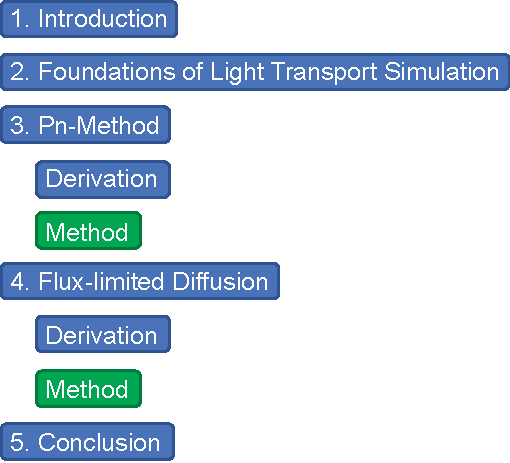
\includegraphics[width=0.6\textwidth]{02_Introduction/figures/fig_organigram.pdf}
\caption{Organigram of this thesis showing original contributions in green.}
\label{fig:intro_organization}
\end{figure}








